\subsubsection{Modelo recurrente básico}

Este modelo es el mismo modelo que el denso pero añadiendo una nueva capa recurrente simple explicada en la sección \ref{rnn_theory}. La capa recurrente simple es una capa que nos permite usar información de otros intervalos anteriores que serán usados para la predicción final. Esta capa recurrente tiene 100 unidades y gráficamente el modelo se puede representar de la siguiente forma:
\begin{figure}[H]
    \centering
    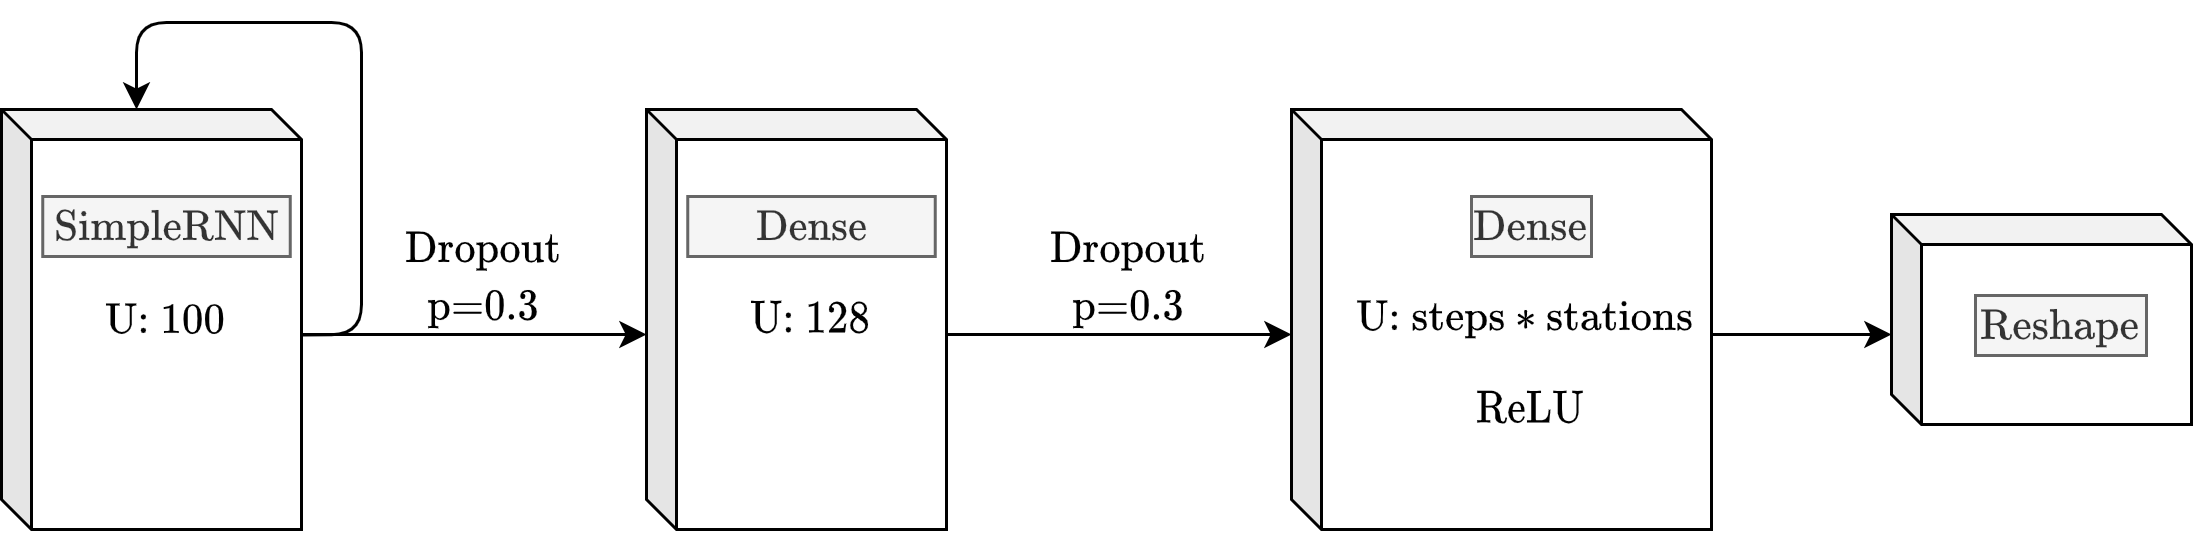
\includegraphics[width=12cm]{images/solution/models/simpleRnn.png}
    \caption{Modelo recurrente básico}
    \label{fig:dense-model}
\end{figure}

Como se puede observar es una extensión del modelo denso explicado en la sección anterior pero añadiendo una nueva capa de tipo \textit{SimpleRNN}. El código de este modelo se ha definido como se muestra a continuación:
\begin{minted}[fontsize=\scriptsize]{python}
from tensorflow.keras.models import Sequential
from tensorflow.keras.layers import Reshape, Dense, Dropout, Lambda, SimpleRNN

# `steps` is a variable which has the number of intervals to be predict
steps = 0 

# `stations` is the number of stations in the bike network
stations = 0

rnn_model = Sequential([
    # Matrix to vector
    Lambda(lambda x: x[:, -1:, :]),
    
    SimpleRNN(100, return_sequences=True),
    
    Dropout(0.3),
    Dense(128),
    Dropout(0.3),
    
    # Ouput layer
    Dense(steps * stations),
    
    # Vector to matrix
    Reshape([steps, stations])
])
\end{minted}


Los resultados del modelo se pueden ver junto al resto de resultados en la sección \ref{results}.